\chapter{Rekursive Strukturen und die natürlichen Zahlen}

%\section*{Prolog}



\section*{Relevanz für die Informatik}
\begin{itemize}
\item Rekursion ist ein wichtiges Sprachelement von höheren Programmiersprachen (absolut zentral für funktionale Sprachen).
\item Induktion kann verwendet werden, um die  Korrektheit von rekursiven Programmen zu beweisen.
\item Rekursion und Induktion sind von fundamentaler Bedeutung für die theoretische Informatik (rekursive Funktionen, verallgemeinerter Rekursionsbegriff)
\item Informatik ist voll von ``induktiven Definitionen'' (Syntax und Semantik von Programmiersprachen, primitiv rekursive Funktionen uvm.).
\end{itemize}



\section*{Lernziele}
Sie kennen die
\begin{itemize}
\item Peano-Axiome und verstehen deren Bedeutung.
\item Die Begriffe von Induktion und Rekursion
\end{itemize}
Sie verstehen
\begin{itemize}
\item wie Induktion und Rekursion zusammenhängen.
\item wie man rekursiv eine Funktion definieren kann und wie diese Definitionsweise zu rechtfertigen ist.
\item wie sich die arithmetischen Operationen rekursiv aus der Nachfolgerabbildung definieren lassen.
\item wie die üblichen Rechenregeln für natürliche Zahlen aus den Peano-Axiomen folgen.
\end{itemize}
Sie sind in der Lage
\begin{itemize}
\item Induktionsbeweise zu führen.
\item Algorithmen und Problemlösungsstrategien durch Rekursion zu beschreiben.
\item Probleme zu erkennen, die sich effektiv durch Rekursion lösen lassen.
\end{itemize}


\section*{Literatur und Links}
\begin{itemize}
\item Aufgaben mit Lösungen zu Induktion:\\ \url{http://www.emath.de/Referate/induktion-aufgaben-loesungen.pdf}
\item Erklärungen zu Induktion:\\
Appendix B von \url{https://slc.openlogicproject.org/slc-screen.pdf}
\item Wikipedia Einträge zu Induktion und Rekursion:\\
\url{http://de.wikipedia.org/wiki/Vollst%C3%A4ndige_Induktion}\\
\url{http://de.wikipedia.org/wiki/Rekursion}
\end{itemize}


\section{Die grundlegende Struktur der natürlichen Zahlen}
Wir haben die Menge $\N$ bereits kennen und als Grundlage für viele Beispiele auch schätzen gelernt. In diesem Kapitel möchten wir diese Menge etwas genauer verstehen, wir wollen ihre innere Struktur (Ordnung und Operationen) untersuchen. Ausgangspunkt für unsere Betrachtungen ist die Anschauung der natürlichen Zahlen als eine auf dem ``Zahlenstrahl'' angeordnete, diskrete Menge:

\begin{center}
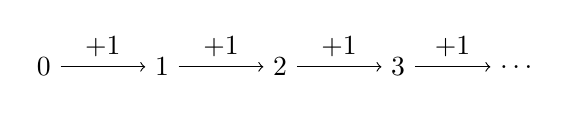
\begin{tikzpicture}[scale=1.5]
  \node (0) at (0,0) {$0$};
  \node (1) at (1,0) {$1$};
  \node (2) at (2,0) {$2$};
  \node (3) at (3,0) {$3$};
  \node (4) at (4,0) {$\dots$};
  \path[->] (0) edge node[above] {$+1$} (1)
  			(1) edge node[above] {$+1$} (2)
  			(2) edge node[above] {$+1$} (3)
  			(3) edge node[above] {$+1$} (4);
\end{tikzpicture}
\end{center}

 Von dieser Anschauung geleitet, listen wir nun einige Grundtatsachen über die Struktur $\N$ auf. Diese Grundannahmen entsprechen den sogenannten \textit{Peano-Axiomen}.

\begin{itemize}
 \item Die Zahl $0$ ist eine natürliche Zahl. Jede natürliche Zahl $k$ hat genau einen Nachfolger $k+1$. Der Nachfolger jeder natürlichen Zahl ist wiederum eine natürliche Zahl.
 \item Die Zahl $0$ ist die einzige natürliche Zahl, die kein Nachfolger ist:
 \[
 \forall n\in\N\,(\underbrace{\forall k\in\N\,(n\neq k+1)}_{n\text{ ist kein Nachfolger}}\Leftrightarrow n=0 ).
 \]
 \item Jede natürliche Zahl ist Nachfolger von höchstens einer natürlichen Zahl:
 \[
 \forall n,m\in\N\,(n+1=m+1\Rightarrow n=m).
 \]
\item \textit{Das Prinzip der (vollständigen) Induktion}: Es sei $A(n)$ eine Eigenschaft (ein Prädikat) von natürlichen Zahlen. Aus den beiden Voraussetzungen
\begin{itemize}
\item[] \textbf{Induktionsverankerung (I.V.):} $A(0)$
\item[] \textbf{Induktionsschritt (I.S.):} $\forall n\in \N\,(A(n)\Rightarrow A(n+1))$,
\end{itemize}
folgt die Gültigkeit von $\forall n\in\N\,(A(n))$.
\end{itemize}

\begin{rk}
Der Induktionsschritt ist stets von der Form
\[
\forall n\in\N\,\big( \underbrace{A(n)}_{\text{Induktionsannahme}}\,\Rightarrow A(n+1)\,\big)
\]
für ein Prädikat $A$. Der Teil $A(n)$ wird dabei \textit{Induktionsannahme} genannt, weil er beim Nachweis von $A(n+1)$ als Annahme verwendet werden darf.
\end{rk}

\begin{rk}
Das Prinzip der vollständigen Induktion ist ein mächtiges Mittel um viele verschiedene Behauptungen über natürliche Zahlen beweisen zu können. Will man eine Aussage von der Form
\[
\text{Jede natürliche Zahl }n\text{ erfüllt }E(n)
\]
für ein Prädikat $E$ beweisen, dann muss man, wenn man die Eigenschaft $E$ nicht für alle natürlichen Zahlen \textit{simultan} beweisen kann, im Prinzip unendlich viele Schritte bewältigen:
\begin{enumerate}
\item[1.] Schritt: Zeige $E(0)$.
\item[2.] Schritt: Zeige $E(1)$.
\item[3.] Schritt: Zeige $E(2)$.
\item[$\vdots$]
\end{enumerate}
Die Stärke des Induktionsargumentes liegt nun  darin, all diese unendlich vielen Schritte auf zwei Schritte zu reduzieren:
\begin{enumerate}
\item[1.] Schritt (I.V.): Zeige $E(0)$.
\item[2.] Schritt (I.S.): Zeige, dass die Eigenschaft $E$ unter Nachfolgern erhalten bleibt. Intuitiv könnte man sagen, dass die Eigenschaft $E$ von jeder natürlichen Zahl auf die nächste ``vererbt'' wird.
\end{enumerate}
\end{rk}

\begin{bsp}
Wir betrachten die Eigenschaft $A(n)$, die besagt, dass die Summe aller natürlichen Zahlen bis $n$ halb so gross wie die Zahl $n(n+1)$ ist:
\[
0+1+\dots+n =\frac{n(n+1)}{2}.
\]
Wir beweisen nun per Induktion nach $n$, dass die Eigenschaft $A(n)$ für jede natürliche Zahl $n$ zutrifft.
\begin{proof}
Wir zeigen zuerst die Induktionsverankerung:
\begin{itemize}
\item \textbf{Verankerung ($n=0$):} $A(0)$ gilt, weil
\[
0=\frac{0\cdot 1}{2}
\]
offensichtlich korrekt ist.
\item \textbf{Schritt ($n\to n+1$):} Für den Induktionsschritt müssen wir zeigen, dass für jede natürliche Zahl $n$ mit der Eigenschaft $A(n)$ auch $A(n+1)$ gilt. Wir nehmen dazu an, dass $n$ eine beliebige solche natürliche Zahl sei und betrachten
\begin{align*}
0+1+\dots +n+(n+1)&=(0+1+\dots +n)+(n+1)\\
&\stackrel{A(n)}{=}\frac{n(n+1)}{2}+(n+1)\\
&=\frac{n(n+1)+2(n+1)}{2}\\
&=\frac{(n+1)(n+2)}{2}.
\end{align*}
Daraus folgt der Induktionsschritt.
\end{itemize}
\end{proof}
\end{bsp}

\begin{bsp}
Wir benützen ein Induktionsargument um zu beweisen, dass alle natürlichen Zahlen $n>1$ für beliebige reelle Zahlen $r>-1, r\neq 0$ die folgende Eigenschaft haben:
\[
 (1+r)^n>1+nr.
\]
\begin{proof}~
\begin{itemize}
\item \textbf{Verankerung $(n=2)$:} Die Verankerung gilt, wegen
\[
(1+r)^2=1+2r+r^2>1+2r.
\]
\item \textbf{Schritt $(n\to n+1)$:} Wir nehmen nun an, dass die Aussage für $n$ gilt (I.A.) und zeigen sie für $n+1$:
\begin{align*}
(1+r)^{n+1}&=(1+r)^n(1+r)\\
&\stackrel{I.A.}{>}(1+nr)(1+r)\\
&=1+nr+r+\underbrace{nr^2}_{\text{positiv}}\\
&>1+(n+1)r.\qedhere
\end{align*}
\end{itemize}
\end{proof}
\end{bsp}

\begin{bsp}
Für jede endliche Menge $X$ gilt
\[
|\mathcal{P}(X)|=2^{|X|}.
\]
\begin{proof}
Wir führen den Beweis durch Induktion nach der Anzahl Elemente der Menge $X$.
\begin{itemize}
\item \textbf{Verankerung ($|X|=0$):} Die einzige Menge mit $0$ Elementen ist die leere Menge, es gilt also wie gewünscht
\[
|\mathcal{P}(X)|=|\mathcal{P}(\varnothing)|=|\{\varnothing\}|=1=2^0=2^{|X|}.
\]
\item \textbf{Schritt:} Es sei nun $X$ eine $n+1$ elementige Menge. Aufgrund der Induktionsannahme können wir davon ausgehen, dass für alle Mengen $Y$ mit $n$ Elementen die Gleichung
\[
|\mathcal{P}(Y)|=2^{|Y|}
\]
 erfüllt ist. Da $X\neq\varnothing$ gilt, können wir ein $x\in X$ auswählen. Wir unterteilen die Potenzmenge von $X$ in zwei disjunkte, gleich grosse Teile $A$ und $B$:
 \begin{align*}
 A=\{Y\subseteq X\mid x\notin Y \}\\
 B=\{Y\subseteq X\mid x\in Y \}.
 \end{align*}
Es gilt:
\begin{align*}
|\mathcal{P}(X)|&=|A\cup B|=|A|+|B|\\
&=|A|+|A|=2|A|=2|\mathcal{P}(X\setminus\{x\})|\\&\stackrel{I.A.}{=}2\cdot2^n=2^{n+1}.\qedhere
\end{align*}
\end{itemize}
\end{proof}
\end{bsp}

\begin{satz}[Vollständige Induktion mit Mengen]\label{satz:mengeninduktion}
Für jede Menge $X$ von natürlichen Zahlen gilt: Wenn $X$ die Bedingungen
\begin{itemize}
\item Induktionsverankerung: $0\in X$
\item Induktionsschritt: $\forall n\,(n\in X\Rightarrow n+1\in X)$
\end{itemize}
erfüllt, dann ist bereits $X=\N$.
\end{satz}
\begin{proof}
Ist $E(n)$ das Prädikat $n\in X$, dann folgt mit vollständiger Induktion sofort $\forall n\, (E(n))$ und somit $\N=X$.
\end{proof}

\begin{df}
Die Ordnung $\leq$ auf den natürlichen Zahlen ist durch
\[
x\leq y:\Leftrightarrow \exists k\in\N\,(x+k=y)
\]
gegeben. Wir schreiben weiter
\[
x<y:\Leftrightarrow x\leq y\land x\neq y.
\]
\end{df}
\begin{rk}
Wird die Zahlengerade der natürlichen Zahlen vertikal aufgezeichnet, dann ist sie ein Hasse-Diagramm für die Ordnung $\leq$ auf $\N$.
\begin{center}
\begin{tikzpicture}[scale=1]
  \node (0) at (0,0) {$0$};
  \node (1) at (0,1) {$1$};
  \node (2) at (0,2) {$2$};
  \node (3) at (0,3) {$\vdots$};
  \draw (0)--(1)--(2)--(3);
\end{tikzpicture}
\end{center}
\end{rk}


\begin{satz}\label{satz:minimumprinzip}
Jede nichtleere Menge von natürlichen Zahlen hat ein minimales Element.
\end{satz}
\begin{proof}
Wir zeigen, dass jede Menge von natürlichen Zahlen, die kein minimales Element enthält, leer ist. Dazu wählen wir eine beliebige Menge $X\subseteq\N$ ohne minimales Element. Um zu zeigen, dass die Menge $X$ leer ist, genügt es zu zeigen, dass die Menge
\[
Y=\{n\in\N\mid \forall x\in X\,(n<x) \}
\]
aller natürlichen Zahlen, die ``unterhalb'' von $X$ liegen, bereits alle natürlichen Zahlen enthält. Wir zeigen $Y=\N$ mithilfe von Satz~\ref{satz:mengeninduktion}.
\begin{itemize}
\item \textbf{Verankerung:} Es gilt $0\in Y$, weil sonst $0$ das minimale Element von $X$ wäre, was unserer Wahl von $X$ widerspricht.
\item \textbf{Induktionsschritt:} Ist $n\in Y$, dann gilt für alle Elemente $x$ von $X$ die Ungleichung $n<x$. Es gilt daher $n+1\leq x$ für alle Elemente $x$ von $X$. Da $n+1$ kein minimales Element von $X$ sein kann, gilt daher $n+1\in Y$.
\end{itemize}
Aus Satz~\ref{satz:mengeninduktion} folgt nun, dass $Y=\N$ und somit wie gewünscht $X=\varnothing$ ist.
\end{proof}

\begin{satz}\label{satz:descendingchains}
Es gibt keine unendlich absteigende Folge
\[
a_0>a_1>\dots >a_n>a_{n+1}>\dots
\]
von natürlichen Zahlen.
\end{satz}
\begin{proof}
Gäbe es eine absteigende Folge
\[
a_0>a_1>\dots >a_n>a_{n+1}>\dots,
\]
dann hätte die Menge
\[
\{
a_0,a_1,\dots,a_n,a_{n+1},\dots \}
\]
kein minimales Element. Dies widerspricht Satz~\ref{satz:minimumprinzip}.
\end{proof}

Aus den eben bewiesenen Sätzen können wir neue Beweismethoden herleiten:

\begin{rk}[Der kleinste Verbrecher]
Die Beweismethode des ``kleinsten Verbrechers'' geht wie folgt: Will man zeigen, dass alle natürlichen Zahlen eine Eigenschaft $E$ haben, dann geht man davon aus, dass wenn dies nicht der Fall wäre, es eine kleinste natürliche Zahl $n_0$ (den kleinsten Verbrecher) gäbe, die \textit{nicht} die Eigenschaft $E$ hat. Führt man diese Annahme zu einem Widerspruch, so hat man die ursprüngliche Behauptung bewiesen. Obwohl die Methode des ``kleinsten Verbrechers'' also nichts anderes als die Kombination eines Widerspruchsargumentes mit Satz~\ref{satz:minimumprinzip} ist, handelt es sich doch um eine sehr ``anwenderfreundliche'' und einprägsame Beschreibung dieser Argumentationsfolge.
\end{rk}

\begin{bsp}
Wir benützen die Methode des ``kleinsten Verbrechers'' um zu beweisen, dass jede natürliche Zahl, die mindestens zwei Teiler hat, mindestens einen Primfaktor besitzt (von einer Primzahl geteilt wird).
\begin{proof}
Es sei $n_0$ die kleinste natürliche Zahl mit mindestens zwei Teilern, die keine Primfaktoren besitzt (der ``kleinste Verbrecher''). Da $n_0$ keine Primfaktoren hat, ist $n_0$ selbst auch keine Primzahl und es gilt $n_0\neq 0$. Es folgt somit, dass ein Teiler $1<x<n_0$ von $n_0$ existieren muss. Da $1<x$ gilt, hat $x$ mindestens zwei Teiler ($1$ und $x$) und somit, wegen $x<n_0$, einen Primfaktor $p$. Da die Teilbarkeitsrelation transitiv ist, muss $p$ aber auch ein Primfaktor von $n_0$ sein. Dies ist der gesuchte Widerspruch.
\end{proof}
\end{bsp}

\begin{ueb}
	Beweisen Sie mit der Methode des ``kleinsten Verbrechers''.
	Jede natürliche Zahl von der Form ($n^2+n$) ist gerade.
\end{ueb}
\begin{lsg}
	\ifthenelse{\boolean{ml}}{
		Wir nehmen an, dass es ungerade natürliche Zahlen von der Form $n^2+n$ gibt. Die Zahl $n^2+n$ sei die kleinste solche Zahl (der kleinste Verbrecher). Weil $n$ nicht Null sein kann (sonst wäre $n^2+n$ gerade), muss es ein $k\in \N $ mit $n=k+1$ geben. Weil $k<n$ gilt, muss $k^2+k$ aber gerade sein. Daraus folgt
		\begin{align*}
			n^2+n &= (k+1)^2+(k+1)= k^2 + 2k + 1 + k + 1\\
			&= \underbrace{k^2+k}_{gerade}+\underbrace{2k+2}_{gerade}
		\end{align*}
		und somit, dass $n^2+n$ gerade ist (im Widerspruch zur Annahme). }{~
		\answerspace{14cm}}
\end{lsg}

\ifthenelse{\boolean{ml}}{\newpage}{}
\section{Vom Induktionsbeweis zum rekursiven Algorithmus}

\begin{bsp}[Türme von Hanoi]~
\begin{center}
\includegraphics[width=0.8\textwidth]{figures/hanoi}
\end{center}
\begin{quote}
``Die Türme von Hanoi''\footnote{Beschreibung und Bild von Wikipedia.} ist ein Geduldspiel. Das Spiel besteht aus drei gleich grossen Stäben A, B und C, auf die mehrere gelochte Scheiben gelegt werden, alle verschieden gross. Zu Beginn liegen alle Scheiben auf Stab A, der Grösse nach geordnet, mit der grössten Scheibe unten und der kleinsten oben. Ziel des Spiels ist es, den kompletten Scheiben-Stapel von A nach C zu versetzen.
Bei jedem Zug darf die oberste Scheibe eines beliebigen Stabes auf einen der beiden anderen Stäbe gelegt werden, vorausgesetzt, dort liegt nicht schon eine kleinere Scheibe. Folglich sind zu jedem Zeitpunkt des Spieles die Scheiben auf jedem Feld der Grösse nach geordnet.
\end{quote}
Wir wollen beweisen, dass ``die Türme von Hanoi'' mit beliebig vielen Scheiben erfolgreich gespielt werden können.
\begin{proof} Wir benutzen ein Induktionsargument ($n$ sei die Anzahl Scheiben):
\begin{itemize}
\item \textbf{Verankerung $n=0$:} Dieser Fall ist trivial, da es keine Scheiben zu bewegen gibt.
\item \textbf{Induktionsschritt $n\to n+1$:} Wir betrachten das Spiel mit $n+1$ Scheiben. Nach Induktionsvoraussetzung gibt es eine Lösungsstrategie für das Spiel mit nur $n$ Scheiben. Diese Strategie können wir offensichtlich dazu verwenden, um alle bis auf die grösste Scheibe auf den Stab B zu verschieben. Nun können wir die grösste Scheibe auf den Stab $C$ verschieben, um anschliessend nochmal die Strategie für das Spiel mit $n$ Scheiben anzuwenden und alle kleineren Scheiben auf den Stab C zu bewegen. Das Spiel ist somit auch für $n+1$ Scheiben lösbar. \qedhere
\end{itemize}
\end{proof}
\begin{rk}
Der Beweis, dass die Türme von Hanoi für beliebige $n$ gelöst werden können, ist mehr als nur eine Argumentationskette, die dazu geeignet ist jemanden davon zu überzeugen, dass es tatsächlich \textit{irgendwie möglich sein muss} das Spiel zu gewinnen. Es steckt viel mehr in diesem Beweis; der Beweis gibt einen konkreten Algorithmus (rekursiv) vor, wie das Spiel erfolgreich gespielt werden kann. Wir betrachten eine Implementierung dieser Lösungsstrategie in Java.


\lstset{language=Java}
\begin{framed}
\begin{lstlisting}
// x-viele Scheiben von A nach B verschieben:
// Falls x=0, dann ist nichts zu tun.
// Sonst, zuerst die oberen (x-1) Scheiben von A nach C
// verschieben,
// dann die groesste Scheibe von A nach B verschieben
// und schliesslich alle anderen Scheiben von C nach B
// verschieben
public class HanoiSolver{

    public String solve(int size){
        return AC(size);
    }

    private String AB(int x){
        if (x==0) return "";
        return AC(x-1)+" AB "+CB(x-1);
    }

    private String AC(int x){
            if (x==0) return "";
            return AB(x-1)+" AC "+BC(x-1);
    }

    private String BC(int x){
            if (x==0) return "";
            return BA(x-1)+" BC "+AC(x-1);
    }

    private String BA(int x){
            if (x==0) return "";
            return BC(x-1)+" BA "+CA(x-1);
    }

    private String CB(int x){
            if (x==0) return "";
            return CA(x-1)+" CB "+AB(x-1);
    }

    private String CA(int x){
            if (x==0) return "";
            return CB(x-1)+" CA "+BA(x-1);
    }
}
\end{lstlisting}
\end{framed}
und die kurze Fassung:
\begin{framed}
\begin{lstlisting}
public class HanoiSolverCompact{

    public String solve(int size){
        return hanoi("A","C","B",size);
    }

    private String hanoi(String x,String y,String z,int n){
        if(n==0) return "";
        return hanoi(x,z,y,n-1)+" "+x+y+hanoi(z,y,x,n-1);
    }
}
\end{lstlisting}
\end{framed}

%\begin{lstlisting}
%let rec AB x =
%    if x=0 then []
%    else (CB (x-1))@(('A','B')::(AC (x-1)))
%
%and AC x =
%    if x=0 then []
%    else (BC (x-1))@(('A','C')::(AB (x-1)))
%
%and BC x =
%    if x=0 then []
%    else (AC (x-1))@(('B','C')::(BA (x-1)))
%
%and BA x =
%    if x=0 then []
%    else (CA (x-1))@(('B','A')::(BC (x-1)))
%
%and CB x =
%    if x=0 then []
%    else (AB (x-1))@(('C','B')::(CA (x-1)))
%
%and CA x =
%    if x=0 then []
%    else (BA (x-1))@(('C','A')::(CB (x-1)))
%
%\end{lstlisting}
\end{rk}
\end{bsp}


\begin{bsp}\label{bsp:plättli}
Ist es immer möglich ein ``gelochtes $n\times n$-Quadrat''
\begin{center}
\begin{tabular}{ | c | c | c | c | c  | c | c | c | }
\hline
&&&&&&&\\
\hline
&&&&&&&\\
\hline
&&&&&&&\\
\hline
&&&&&&&\\
\hline
&&&&&&\cellcolor{black}&\\
\hline
&&&&&&&\\
\hline
&&&&&&&\\
\hline
&&&&&&&\\
\hline
\end{tabular}
\end{center}

mit Flächen von der Form
\begin{tabular}{ c c }
&\cellcolor{black}\\
\cellcolor{black}&\cellcolor{black}
\end{tabular}
``passgenau'' zu überdecken? Ja, wenn $n$ eine Zweierpotenz ist. Wir können diese Behauptung durch Induktion wie folgt beweisen:  Wir nehmen an, dass das ``gelochte Quadrat'' eine Seitenlänge von $2^n$ hat.
\begin{itemize}
\item Verankerung ($n=0$): Wenn $n=0$, dann besteht das gelochte Quadrat nur aus einem Loch. Wir können das Quadrat (ohne etwas zu tun) überdecken.
\item Hat das Quadrat die Seitenlänge $2^{n+1}$, dann zerlegen wir es in vier gleich grosse Quadranten, die alle die Seitenlänge $2^n$ haben. Wir platzieren eine der Flächen wie unten angedeutet (rot).
\begin{center}
\begin{tabular}{ | c | c | c | c !{\color{red}\vrule} c  | c | c | c | }
\hline
&&&&&&&\\
\hline
&&&&&&&\\
\hline
&&&&&&&\\
\hline
&&&\cellcolor{red}&\cellcolor{red}&&&\\
\arrayrulecolor{red}\hline
\arrayrulecolor{black}&&&\cellcolor{red}&&&&\\
\hline
&&&&&&\cellcolor{black}&\\
\hline
&&&&&&&\\
\hline
&&&&&&&\\
\hline
\end{tabular}
\end{center}
Nun sind alle Quadranten ein ``gelochtes Quadrat'' der Seitenlänge $2^n$. Wir können also nach Induktionsvoraussetzung alle Quadranten passgenau belegen.
\end{itemize}
\end{bsp}

\begin{ueb}
Implementieren Sie (ausgehend vom Beispiel~\ref{bsp:plättli}) in einer Programmiersprache Ihrer Wahl, einen Algorithmus zur Überdeckung von ``gelochten Quadraten'', die eine Zweierpotenz als Seitenlänge haben.
\end{ueb}

\section{Rekursive Definitionen}

%\begin{df}
%Eine Menge $X\subseteq \N$ bezeichnen wir als initiales Segment von $\N$ falls mit jeder Nachfolgerzahl\footnote{Eine Nachfolgerzahl ist eine natürliche Zahl die ungleich Null ist} $N(n)=n+1$ welche in $X$ liegt auch deren Vorgänger $n$ ein Element von $X$ ist. Etwas formaler aufgeschrieben ist also $X\subseteq \N$ eine initiale Teilmenge von $\N$ falls die Eigenschaft
%\[
% \forall n\in\N\,\big( n+1\in X\Rightarrow n\in X \big)
%\]
%auf $X$ zutrifft.
%\end{df}

%\begin{bsp}
%Alle Mengen von der Form $\N_{<k}$ mit einer natürlichen Zahl $k$ sind initiale Teilmengen von $\N$. Die %Menge $\N$ selbst ist ebenfalls eine initiale Teilmenge von $\N$.
%\end{bsp}

%\begin{rk}
% Jede nichtleere initiale Teilmenge von $\N$ enthält das Element $0$.
%\end{rk}
%\begin{proof}
 %Sei $M$ folgende Teilmenge von $\N$:
 %\[
 % M:=\{n\in\N\mid \text{es gibt ein initiales Segment }S\text{ mit }0\notin S\text{ und } n\in S\}
% \]
%Wir wollen zeigen, dass $M$ keine Elemente besitzt wir tun dies in dem wir zeigen, dass die Menge $X:=\N\backslash M$ alle natürlichen Zahlen enthält. Wir benützen das Prinzip der vollständigen Induktion. Wäre $0$ nicht in $X$, so wäre $0$ in $M$ dann gäbe es aber ein initiales Segment $S$ mit gleichzeitig $0\in S$ und $0\notin S$, ein Widerspruch. Also ist $0\in X$. sei weiter $n\in X$ dann ist $n\notin M$, es gibt also kein initiales Segment $S$ mit $n\in S$ und $0\notin S$. Gäbe es nun ein initiales Segment $S$ mit $0\notin S$ und $n+1\in S$, dann müsste (da $S$ initial ist) auch $n\in S$ sein woraus aber wieder $n\in M$ folgen würde. Also kann solch ein $S$ nicht existieren und folglich ist $n+1\in X$. Insgesamt habe wir also $X=\N$. Somit kann ein Initiales Segment welches die Null nicht enthält überhaupt keine Elemente enthalten.
%\end{proof}

Rekursive Definitionen bezeichnen die mathematisch einwandfreie Art, ein Objekt durch Bezugnahme (Selbstreferenz) auf das zu definierende Objekt selbst zu definieren.

\begin{bsp}
Ein Palindrom ist ein Wort, das rückwärts und vorwärts gelesen gleich lautet. Beispiele von Palindromen sind $yxy,acaca,arbbra,b,a,\dots$. Obwohl es uns anschaulich klar ist, welche Wörter Palindrome sind und welche nicht, ist unsere Beschreibung keine mathematisch präzise Definition. Dies wird insbesondere dann offensichtlich, wenn wir ein Programm schreiben müssen (ohne ``String-umkehrende'' Operatoren benützen zu dürfen), das von einem gegebenen Wort (String) entscheidet ob dieses ein Palindrom ist oder nicht. Wie können wir also Palindrome definieren (eindeutig beschreiben), ohne auf unsere Vorstellung von rückwärts und vorwärts lesen angewiesen zu sein? Durch Rekursion:\\
Ein Wort $w$ ist ein Palindrom, wenn mindestens eine der beiden folgenden Bedingungen erfüllt ist:
\begin{itemize}
\item Das Wort $w$ besteht aus einem oder gar keinem Buchstaben (Länge von $w$ $<2$).
\item Es gibt einen Buchstaben (Zeichen, Char) $x$ und ein $\underbrace{Palindrom}_{Selbstreferenz}$ $u$ so, dass $w=xux$ gilt.
\end{itemize}
Obwohl diese Definition, durch die in ihr vorhandenen Selbstreferenz, ein wenig ``obskur'' erscheinen mag, können wir sie direkt in ein Computerprogramm übersetzen.\\
In Java:

\lstset{language=Java}
\begin{framed}
\begin{lstlisting}
 boolean palindrome(String w){
     if (w.length() < 2) return true;
     int last = w.length()-1;
     char a = w.charAt(0);
     char b = w.charAt(last);
     if (a == b) return palindrome(w.substring(1, last-1));
     return false;
 }
\end{lstlisting}
\end{framed}
\end{bsp}

\begin{thrm}[Rekursive Definitionen]\label{thrm:rekursive definitionen}
 Ist $M$ eine Menge und $G:M\times\N\rightarrow M$ sowie $c\in M$, dann gibt es eine eindeutig bestimmte Funktion $F:\N\rightarrow M$, welche die Gleichungen (Rekursionsgleichungen)
\begin{align*}
 F(0)&=c\\
F(k+1)&=G(\underbrace{F(k)}_{Selbstbezug},k)
\end{align*}
erfüllt.
\end{thrm}
\begin{proof}[Beweisidee]
Die Behauptung besteht aus einer Eindeutigkeitsaussage und einer Existenzaussage:
\begin{itemize}
\item Die Funktion $F:\N\to M$ ist durch die Rekursionsgleichungen eindeutig bestimmt. Das heisst, dass es keine andere  Funktion gibt, die den Rekursionsgleichungen von $F$ genügt.
\item Es gibt überhaupt eine Funktion, die den Rekursionsgleichungen genügt.
\end{itemize}
Wir beweisen zuerst die Eindeutigkeitsbedingung. Wir nehmen an, dass $F$ und $H$ zwei Funktionen sind, die beide die oben genannten Rekursionsgleichungen erfüllen und zeigen, dass daraus $F=H$ folgt. Es genügt mit Induktion zu zeigen, dass für jede natürliche Zahl $n\in \N$ die Gleichung $F(n)=H(n)$ gilt (weil dann $H=F$ gilt).
\begin{itemize}
\item Verankerung ($n=0$): Aufgrund von
\[
F(0)=c=H(0)
\]
ist die Induktionsverankerung erfüllt.
\item Schritt ($n\to n+1$): Wir nehmen an, dass $F(n)=H(n)$ gilt und müssen $F(n+1)=H(n+1)$ beweisen. Dies folgt sofort aus
\[
F(n+1)=G(F(n),n)\stackrel{IA}{=}G(H(n),n)=H(n+1).
\]
\end{itemize}
Nun kommen wir zur Existenzaussage. Anstelle eines formalen Beweises, wollen wir uns an dieser Stelle bloss anschaulich davon überzeugen, dass eine Funktion $F$ immer existiert. Wir geben einen iterativen Algorithmus (in Pseudocode) an, der die gesuchte Funktion realisiert.
\begin{framed}
\begin{lstlisting}[language=Java]
input(n)
lst=[c] // Eine Liste mit einzigem Eintrag c
for i = 0..(n-1) do
    x = G(lst[i],i)
    lst.add(x) // Den aktuellen Funktionswert zur Liste
               // (aller Funktionswerte) hinzufuegen.
return lst[n]
\end{lstlisting}
\end{framed}\qedhere
\end{proof}
% \begin{rk}
%  Der folgende Beweis ist ziemlich abstrakt, seine Darlegung richtet sich deshalb vor allem an (sehr) interessierte Student(inn)en.
% \end{rk}
% \begin{proof}[Beweis]
%Wir müssen einerseits beweisen, dass bei gegebenem $g:\N\rightarrow M$ und $c\in M$ überhaupt eine Funktion $f:\N\rightarrow M$ existiert welche die Rekursionsgleichungen erfüllt und dann noch zeigen, dass diese eindeutig ist. Wir Beweisen zuerst die \textbf{Eindeutigkeit}. Angenommen, dass es zwei Funktionen $h,f:\N\rightarrow M$ gibt die beide die Rekursionsgleichungen erfüllen, müssen wir zeigen, dass für alle $n\in\N$ die Gleichung $f(n)=h(n)$ gilt. Wir machen einen Induktionsbeweis nach $n$.
%\begin{enumerate}
%\item \textit{Induktionsverankerung:} Es gilt sowohl $f(0)=c$ als auch $h(0)=c$ und somit also $f(0)=h(0)$.
%\item \textit{Induktionsschritt:} Wir können $f(n)=h(n)$ (I.A.) annehmen und müssen $f(n+1)=h(n+1)$ beweisen. Wir betrachten dazu folgende Gleichungen:
%\[
%f(n+1)=g(f(n))\stackrel{I.A.}{=}g(h(n))=h(n+1).
%\]
%\end{enumerate}
%Nun zur \textbf{Existenz} der geforderten Funktion $f$. Seien $g:\N\rightarrow M$ und $c\in M$ gegeben. Für diesen Beweis wollen wir eine Funktion $ h:X\rightarrow M$ als ``gut'' bezeichnen falls $X$ ein initiales Segment von $\N$ ist und für jedes Element $k$ von $X$ die Gleichungen
% \begin{align}\label{glg}
%  h(k)=\begin{cases}
% g(h(n))&\text{ falls }k= n+1 \text{ ein Nachfolger ist}\\
%   c &\text{ falls }k=0.
%  \end{cases}
% \end{align}
% Als nächstes wollen wir mit Induktion zeigen, dass jede natürliche Zahl im Definitionsbereich einer ``guten'' Funktion liegt. Dazu sei $G$ die Menge aller solchen natürlichen Zahlen. Die Zahl $0$ ist in $G$ da die Funktion $h:\{0\}\rightarrow M$ mit $h(0)=c$ eine ``gute'' Funktion ist. Wir nehmen nun an $k$ sei in $G$ und müssen zeigen, dass dann auch $ k+1 \in G$ ist. Da $k$ ein Element von $G$ ist, gibt es also ein initiales Segment $X$ von $\N$ mit $k\in X$ und eine ``gute'' Funktion $h:X\rightarrow M$. Wir erweitern nun folgendermassen $h$ zu einer neuen Funktion $\tilde{h}:X\cup\{ k+1 \}\rightarrow M$:
% \begin{align*}
%  \tilde{h}(n)=\begin{cases}
%                h(n)&\text{ falls }n\in X\\
% 	       g(h(k))&\text{ falls }n= k+1 .
%               \end{cases}
% \end{align*}
% Sei nun $n\in X$ beliebig, dann gilt
% \begin{enumerate}
% \item \textit{Fall} $n\neq 0$: Dann ist $n=m+1$ für ein $m\in X$ und somit $\tilde{h}(n)=h(n)=g(h(m))=g(\tilde{h}(m))$.
%  \item \textit{Fall} $n=0$: Dann ist $ \tilde{h}(n)=\tilde{h}(0)=h(0)=c$.
% \end{enumerate}
% Also erfüllt $\tilde{h}$ die Gleichungen (\ref{glg}) für alle Elemente von $X$. Für die natürliche Zahl $ k+1 $ werden die Gleichungen per Definition erfüllt und da $X\cup\{ k+1 \}$ ein initiales Segment von $\N$ ist folgt, dass $ k+1 \in G$  ist. Also ist mit jedem $k$ auch $ k+1 $ im Definitionsbereich einer ``guten'' Funktion. Mit dem Prinzip der vollständigen Induktion können wir also schliessen, dass alle natürlichen Zahlen diese Eigenschaft haben.
%
%Unser nächster Schritt besteht darin, zu zeigen, dass je zwei ``gute'' Funktionen immer kompatibel\footnote{ Zwei Funktionen $f_1,f_2$ heissen kompatibel, falls für alle $x\in dom(f_1)\cap dom(f_2)$ die Gleichung $f_1(x)=f_2(x)$ erfüllt ist. Dies ist genau dann der Fall wenn $f_1\cup f_2$ eine Funktion ist.} sind. Seien also $f_1,f_2$ gute Funktionen mit $f_1:X_1\rightarrow M$ und $f_2:X_2\rightarrow M$. Wir wollen zeigen, dass für jedes $n\in\N$ gilt, dass entweder $n\notin X_1\cap X_2$ oder $f_1(n)=f_2(n)$ gilt. Wir wenden dafür noch einmal das Prinzip der vollständigen Induktion auf $n$ an.
%\begin{enumerate}
%\item \textit{Induktionsverankerung:} Falls $0\in X_1\cap X_2$ gilt, dann folgt aus der Tatsache, dass $f_1,f_2$ gut sind, die Gleichung $f_1(0)=c=f_2(0)$.
%\item \textit{Induktionsschritt:} Es sei $n+1\in X_1\cap X_2$ (sonst gibt es nichts zu zeigen). Weil $X_1$ und $X_2$ initiale Teilmengen von $\N$ sind gilt $n\in X_1\cap X_2$. Aus der Induktionsannahme folgt also $f_1(n)=f_2(n)$, und somit
%\[
%f_1(n+1)=g(f_1(n))\stackrel{I.A.}{=}g(f_2(n))=f_2(n+1)
%\]
%\end{enumerate}
%Nun definieren wir
%\[
%f:=\bigcup_{h\text{ ist gut}}h
%\]
%Weil gute Funktionen paarweise kompatibel sind erhalten wir, dass $f$ eine Funktion ist und weil jede natürliche Zahl im Definitionsbereich einer guten Funktion liegt, dass
%\[
%f:\N\rightarrow M
%\]
%gilt. Wir müssen noch zeigen, dass $f$ den Rekursionsgleichungen genügt. Es sei $h:X\rightarrow M$ eine guten Funktion mit $0\in X$ (eine solche gibt es da jedes $n\in\N$ im Definitionsbereich einer guten Funktion liegt). Es gilt $f(0)=h(0)=c$. Sei nun $n\in\N$ beliebig und $h:X\rightarrow M$ eine gute Funktion mit $n+1\in X$. Weil $X$ eine initiale Teilmenge von $\N$ ist gilt, dass $n$ in $X$ liegt und somit
%\[
%f(n+1)=h(n+1)=g(h(n))=g(f(n)).
%\]
%\end{proof}

\begin{bsp}\label{bsp:rekursive operationen}
Die üblichen arithmetischen Grundoperationen können alle relativ kompakt als rekursive Definitionen geschrieben werden:
\begin{itemize}
\item Die Addition von natürlichen Zahlen:
\begin{align*}
x+0&=x\\
x+(n+1)&=(x+n)+1
\end{align*}
\item Die Multiplikation von natürlichen Zahlen:
\begin{align*}
x\cdot 0 &= 0\\
x\cdot(n+1)&=(x\cdot n)+x
\end{align*}
\item Die Exponentiation von natürlichen Zahlen:
\begin{align*}
x^0&=1\\
x^{n+1}&=x\cdot x^{n}
\end{align*}
\item Die Fakultätsfunktion:
\begin{align*}
0!&=1\\
(n+1)!&=n!\cdot(n+1)
\end{align*}
\item Endliche Summen:
\begin{align*}
\sum_{i=1}^{0}a_i&=0\\
\sum_{i=1}^{n+1}a_{i}&=(\sum_{i=0}^na_i)+a_{n+1}
\end{align*}
\item Endliche Produkte:
\begin{align*}
\prod_{i=1}^{0}a_i&=1\\
\prod_{i=1}^{n+1}a_i&= (\prod_{i=1}^na_i)\cdot a_{n+1}
\end{align*}
\end{itemize}
\end{bsp}
Die üblichen Rechenregeln für natürliche Zahlen lassen sich aufgrund dieser rekursiven Definitionen mit Induktion (und genügend Geduld) beweisen. Wir beschränken uns beispielhaft auf den Beweis von Satz~\ref{satz:partialsummen}.

\begin{ueb}
	Implementieren Sie alle Funktionen von Beispiel \ref{bsp:rekursive operationen} in der Programmiersprache Ihrer Wahl (natürlich ohne Verwendung der vorimplementierten Grundoperationen). Halten Sie sich so präzise wie möglich an die mathematische Definition.
\end{ueb}
\begin{lsg}
	\ifthenelse{\boolean{ml}}{
		Vgl. OLAT ``rekursive Operationen''}{
		Elektronisch zu lösen.}
\end{lsg}

\begin{satz}\label{satz:additionsregeln}
Für alle natürlichen Zahlen $n,m,k$ gelten folgende Rechenregeln für deren Addition:
\begin{enumerate}
\item Neutrales Element: $0+n=n$
\item Kommutativität: $n+m=m+n$
\item Assoziativität: $(n+m)+k=n+(m+k)$
\item Kürzbarkeit: $n+k=m+k\Rightarrow n=m$
\end{enumerate}
\end{satz}


\begin{rk}
Wegen der Assoziativität der Addition, können wir Klammern in endlichen Summen von natürlichen Zahlen weglassen.
\end{rk}




\begin{satz}[Rechenregeln für die Multiplikation]\label{satz:multiplikationsregeln}
Für alle $n,m,k\in\N$ gelten folgende Identitäten\footnote{Wir vereinbaren hier, dass die Multiplikation ``stärker bindet'' als die Addition. Ein Ausdruck von der Form $nm+k$ wird also als $(nm)+k$ interpretiert.}:
\begin{enumerate}
\item \textit{Absorbtion:} $0\cdot n=0$
\item \textit{Neutrales Element:} $1\cdot n=n$
\item \textit{Kommutativität:} $n\cdot m=m\cdot n$
 \item \textit{Assoziativität:} $n\cdot(m\cdot k)=(n\cdot m)\cdot k$
\item \textit{Distributivität:} $n\cdot(m+k)=nm+nk$
\end{enumerate}
\end{satz}
\begin{ueb}
	Nachdem wir die Addition und die Multiplikation rekursiv definiert haben, lassen sich dies in den Sätzen \ref{satz:additionsregeln} und \ref{satz:multiplikationsregeln} geäusserten Tatsachen durch Induktion beweisen. Die einzelnen Beweise sind nicht sonderlich spannend aber eine gute Übung.
\end{ueb}


\begin{satz}[Rechenregeln für Partialsummen]\label{satz:partialsummen}
 Sind $(a_i)_{i\in\N}$ und $(a_i)_{i\in\N}$ beliebige Folgen und ist $c\in\N$, dann gilt für jedes $n\in\N$:
\[
 \sum_{i=1}^n(ca_i+cb_i)=c\big(\sum_{i=1}^na_i+\sum_{i=1}^nb_i\big)
\]
\end{satz}
\begin{proof}
 Induktion nach $n$.
 \begin{itemize}
 \item Verankerung ($n=0$): Die Verankerung gilt aufgrund von
 \begin{align*}
\sum_{i=1}^0(ca_i+cb_i)=0=c(0+0)=c\big(\sum_{i=1}^0a_i+\sum_{i=1}^0b_i\big).
 \end{align*}
 \item Schritt ($n\to n+1$):
 \begin{align*}
\sum_{i=1}^{n+1}(ca_i+cb_i)&=\big(\sum_{i=1}^n(ca_i+cb_i)\big)+(ca_{n+1}+cb_{n+1})\\
&=\big(\sum_{i=1}^n(ca_i+cb_i)\big)+c(a_{n+1}+b_{n+1})\\
&\stackrel{IA}{=}c\big(\sum_{i=1}^na_i+\sum_{i=1}^nb_i\big)+c(a_{n+1}+b_{n+1})\\
&=c\big( \sum_{i=1}^na_i+\sum_{i=1}^nb_i+a_{n+1}+b_{n+1} \big)\\
&=c\big( \sum_{i=1}^na_i+a_{n+1}+\sum_{i=1}^nb_i+b_{n+1} \big)\\
&=c\big( \sum_{i=1}^{n+1}a_i+\sum_{i=1}^{n+1}b_i\big)\qedhere
 \end{align*}
 \end{itemize}
\end{proof}

